\section{Launch loads}
\label{launch_loads}

The launch is a critical part of the mission for the survival of the payload. It is during this period that the payload will experience the most severe loads.
In this section tthe origin and magnitude of these loads will be discussed and their impact on the payload. The mian loads are the quasi-static loads, shock loads, sinusoidal loads, random vibrations, acoustic vibrations.
\\ \\
Quasi-static loads are caused by the engine thrust. The acceleration will increase steadily as the amount of fuel becomes less. Peaks are reached when the engines run out of fuel and stop giving thrust. The ignition of a stage also results in a peak load. These loads are all in the longitudinal direction. There arealso quasi-static loads in the lateral direction caused by ground maneuvres and wind gusts. These kind of loads are expressed as load factors. The maximum load factors for the Soyuz launcher are $+1,5/-5 g$ in longitudinal direction and $+1,8/-1,8 g$ in lateral direction \cite{soyuzman}.
\\ \\
Shock loads are high acceleration loads over a short period of time. They are mostly the result of separation events such as the separation of the boosters, different stages of the launcher and the paayload fairing. They also occur with the deployment of appendages such as the solar panels. The shock response spectrum of some launchers is given in figure \ref{fig:SRS}.

\begin{figure}
\centering
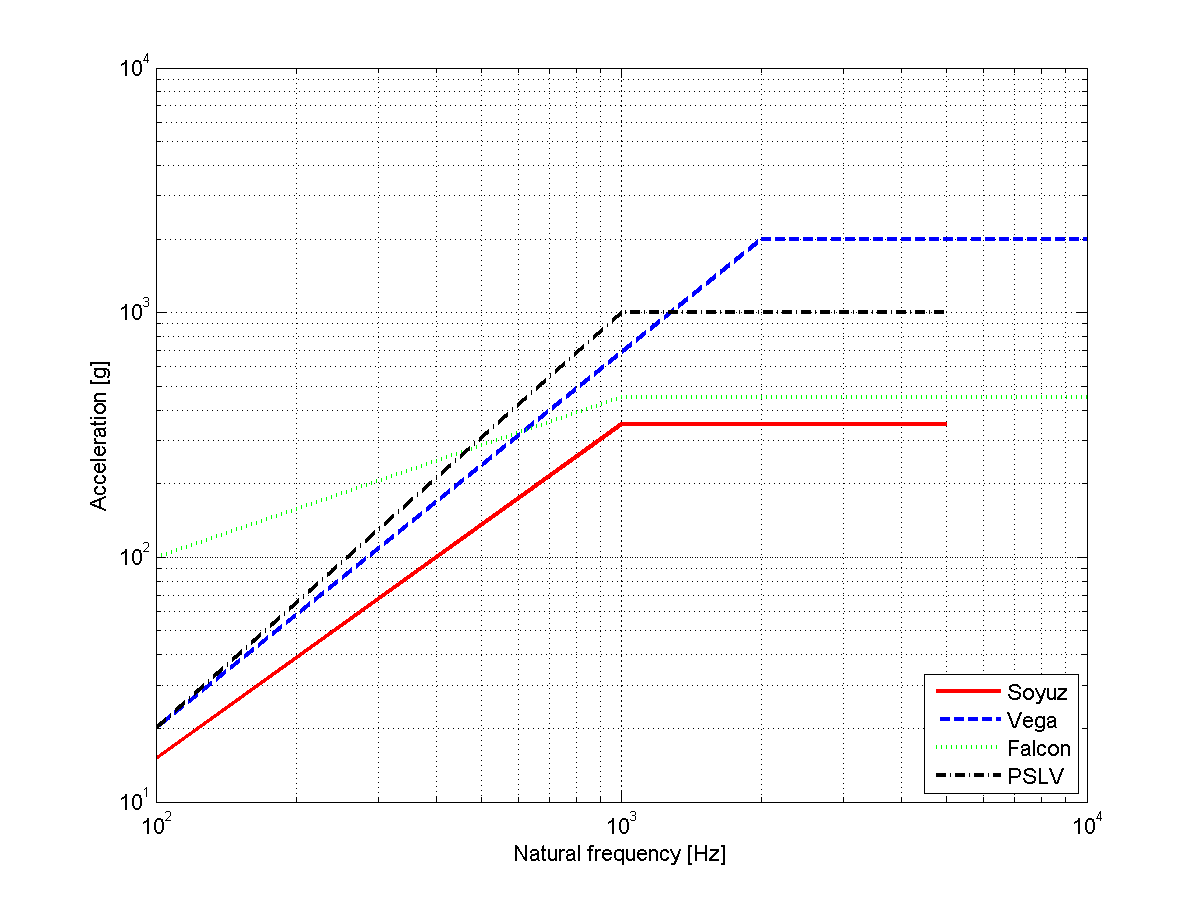
\includegraphics{chapters/img/Shock Loads Acceleration.png}
\caption{Launch shock response spectrum as a function of payload natural frequency}
\label{fig:SRS}
\end{figure}

The release of the payload from the adapter also causes a shock load, but with smaller accelerations that during launch. Ruag space has developed a low-shock release mechanism (CBOD) \cite{ruag}. The CBOD's shock response spectrum is shown in figure \ref{CBOD_SRS}.

\begin{figure}
\centering
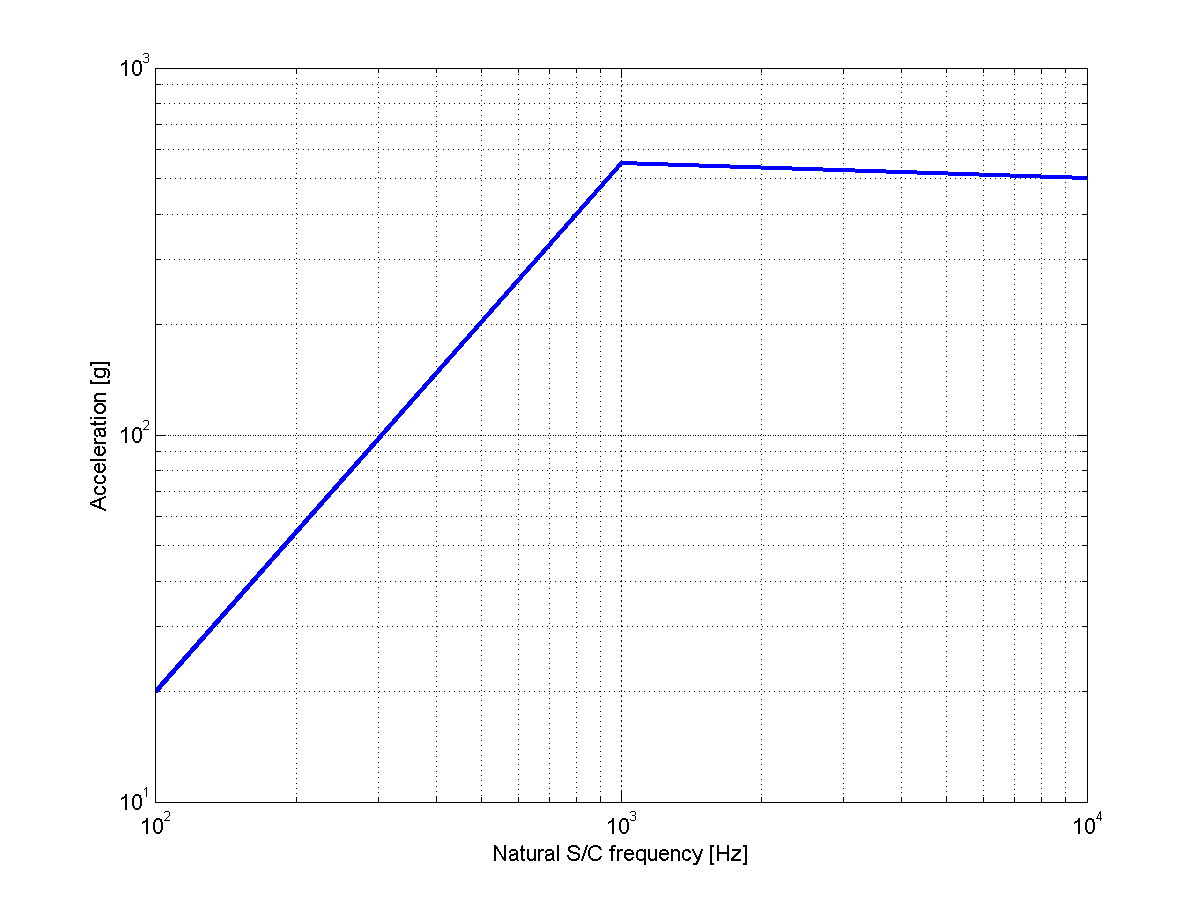
\includegraphics{img/CBOD release acceleration.png}
\caption{Shock response spectrum of the CBOD release mechanism}
\label{fig:CBOD_SRS}
\end{figure}

Another critical load source are random vibrations. For the Soyuz launcher, only random vibrations between 20 and 100 Hz need to be taken in to account because higher frequencies are covered by acoustic vibrations. Random vibrations are caused by the propulsion system and the vibro-acoustic response of the neighbouring structures. Table \ref{tab:random_vibr} gives the power spectral density, root mean square vibration and the duration of the sources for each part of the launch.

\begin{table}[H!]
\centering
\begin{tabular}{ccccc}
\toprule
 Event & \multicolumn{2}{c}{PSD [g^2/Hz]} & $G_{rms} [g]$ & Duration [s] \\
 \midrule
 Frequency band [Hz] & 20 - 50 & 50 - 100 & & \\
 \midrule
 First stage flight & 0.005 & 0.005 - 0.01 & 4.94 & 120 \\
 Second stage flight & 0.0025 & 0.0025 & 3.31 & 480 \\
 Third stage flight & 0.0025 & 0.005 & 3.31 & 480 \\
 Fregat flight & 0.002 & 0.002 & 1.63 & 875 \\
 \bottomrule
 \end{tabular}
 \caption{Soyuz maximum random vibrations}
\label{tab:random_vibr}
\end{table}

Acoustic vibrations are higher than random vibrations, up to 10000 Hz. The main sources are the acoustic noise that radiates from the engines and from aerodynamic turbulence when the launcher passes throug the transsonic part of the flight. During ground operations the venting system also produces noise. For the Soyuz launcher, this does not exceed 94 dB. Apart from the lift-off and the transsonic part of the flight, the acoustic vibrations are rather low. The structures that are affected the most by acoustic loads are structures with a low mass and high surface area, such as solar panels and skins sections. Table \ref{tab:acoustic_vibr} gives the acoustic noise spectrum under the fairing.

\begin{table}[H!]
\centering
\begin{tabular}{cc}
\toprule
Octave Center & Flight limit level [dB]\\
Frequency [Hz] & (reference: 0 dB = 2 X $10^{-5} Pa$ ) \\
\midrule
31.5 & 125\\
63 & 132 \\
125 & 134 \\
250 & 136 \\
500 & 134 \\
1000 & 125 \\
2000 & 121 \\
\bottomrule
 \end{tabular}
 \caption{Soyuz acoustic noise spectrum}
\label{tab:acoustic_vibr}
\end{table}

Sinusoidal loads occur mainly during the atmospheric flight. They are caused by the lift off, bending of the rocket motors, aerodynamic buffeting and oscillations in the propulsions system. To avoid these kind of vibrations, the payload must be constructed in such a way that the payload's natural frequencies will not be close to those of the launcher. This will avoid resonance and thus the payload will experience much lower loads. For the Soyuz launcher it is required that the natural frequencies of the payload will be higher than 15 Hz in lateral direction and higher than 35 Hz in longitudinal direction.